\section{Hagan Rowlenstino A. S (1174040)}
\subsection{Pengertian}
Sistem Informasi Geografis adalah sebuah sistem informasi yang berbasis computer yang dirancang sedemikian rupa untuk bekerja dengan menggunakan data yang memiliki informasi spasial yang bereferensikan keuangan. Sistem ini akan menangkap(capture), mengecek, mengintegrasikan, memanipulasi, menganalisa serta menampilkan data yang secara spasial mereferensikan kondisi bumi.
Menurut ahli :
\begin{enumerate}
	\item Marbel et al (1983), GIS adalah sistem penanganan keruangan
	\item Berry (1988), GIS adalah sistem informasi, referensi internal, serta otomatisasi data keruangan.
\end{enumerate}

4 SUBSISTEM GIS :
\begin{enumerate}
	\item Data Input : mengumpulkan, mempersiapkan, dan menyimpan data spasial dan atributnya dari berbagai sumber
	\item Data output : menampilkan keluaran data dari sistem dalam bentuk tabel, grafik, peta , atau laporan
	\item Data Management : Mengorganisasikan data.
	\item Data Manipulation dan analysis : manipulasi dan permodelan data untuk menghasilkan informasi yang dihasilkan oleh GIS.
\end{enumerate}
Tugas Utama SIG :
\begin{enumerate}
	\item Konversi data dari peta kertas atau foto ke dalalm bentuk digital (digitalizing).
	\item Membuat peta digital.
	\item Memanipulasi atau transformasi agar data – data tersebut kompatibel dengan sistem
	\item Analisis query untuk melihat pola dan trend
	\item Memvisualisasikan hasil dengan peta atau graf
\end{enumerate}
Contoh di beberapa bidang :
\begin{itemize}
	\item SDA : studi kelayakan untuk tanaman pertanian, pengelolaan hutan, dll.
	\item Transportasi : analisis rawan macet dan kecelakaan
	\item Militer : penyediaan data spasial untuk rute perjalanan logistic, peralatan perang, dll.
\end{itemize}

\subsection{Link}
\href{https://www.youtube.com/watch?v=oCACYiDI29s}{Youtube Hagan}
\subsection{Plagiarism}

\begin{figure}[H]
	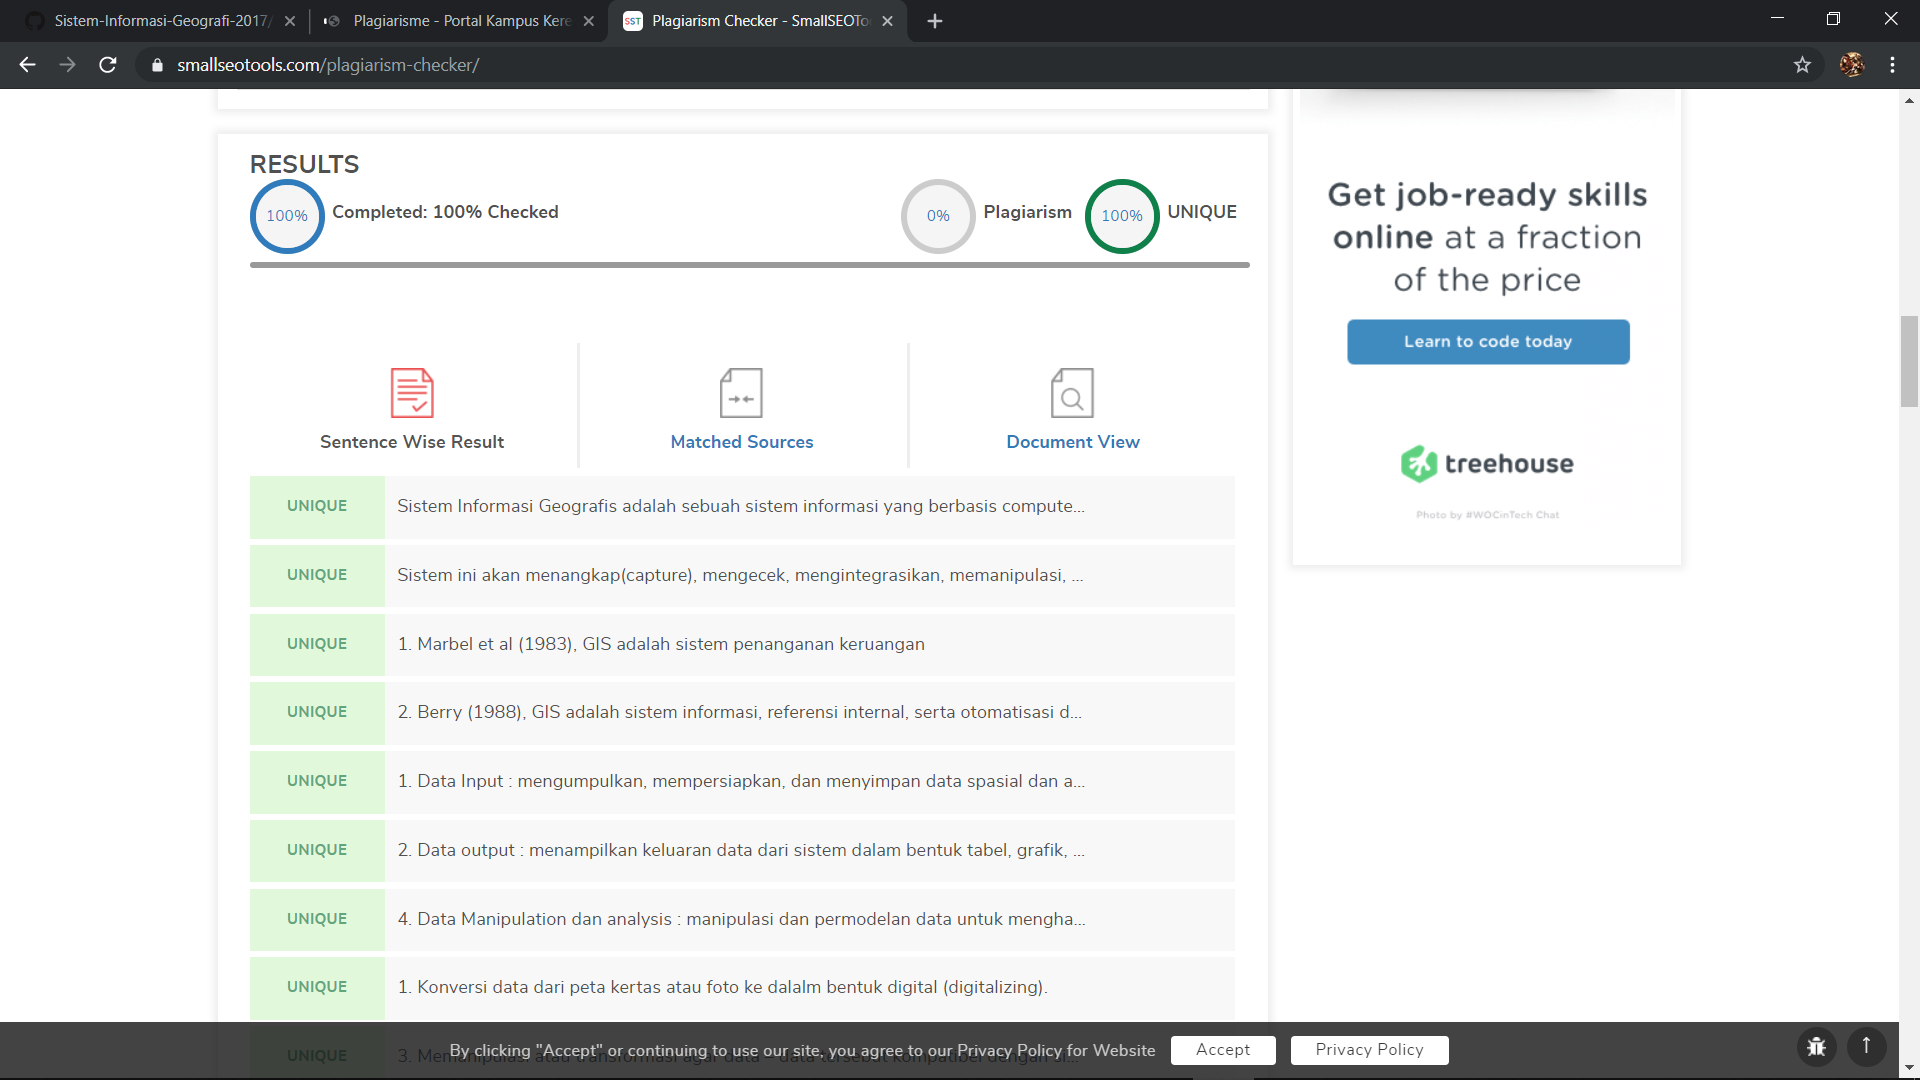
\includegraphics[width=4cm]{figures/1174040/1174040_plagiat_1.png}
	\centering
	\caption{Plagiarisme Hagan}
\end{figure}


